%------------------------------%
%------------------------------%
\chapter{chapitre2}
\markboth{chapitre2}{chapitre2}
%------------------------------%
%------------------------------%


Voir figure \ref{fig:mafigure2}.


\begin{figure}[htbp]
   \begin{center}
      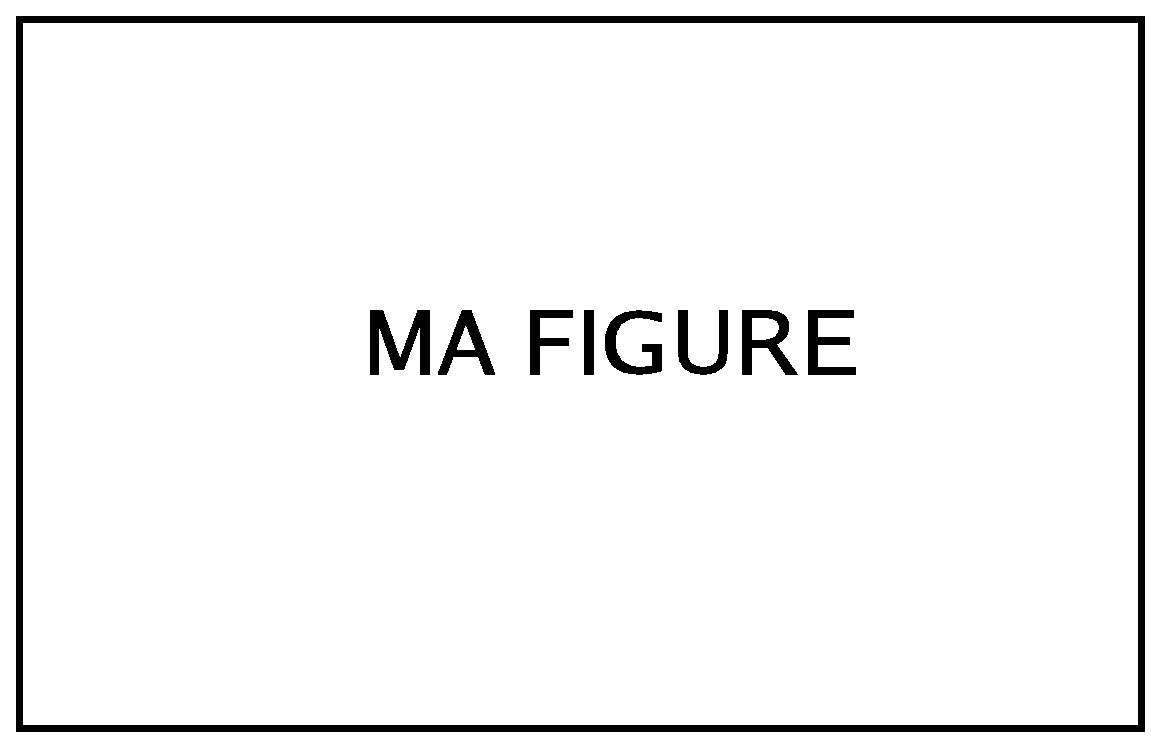
\includegraphics[width=0.8\linewidth]{chapitre2/fig/mafigure.eps}
   \end{center}
   \caption[titre court pour la liste des figures]
   {\footnotesize Titre plus long avec des explications.}
   \label{fig:mafigure2}
\end{figure}
